\section{Case Study: SpaceMaker}
\label{sec:spacemaker}

SpaceMaker is a local-first desktop application that backs up phone media over Wi-Fi or ADB, converts it to AVIF/AV1/H.264 and serves a gallery to phones on the LAN. It is built with FastAPI, an embedded web UI and Qt WebEngine/pywebview, with hexagonal architecture and spec-driven development with six phase gates. Table~\ref{tab:sm} gives its scale.

\begin{table}[h]
\caption{SpaceMaker at the time of writing (2026-10-03).}
\label{tab:sm}
\small
\begin{tabular}{@{}lr@{}}
\toprule
Tracked files & 453 \\
Python / JS+TS / HTML+CSS (lines) & 22.0k / 9.7k / 9.6k \\
Test files / test functions & 101 / 514 \\
Specifications (\code{SPEC.md}) / wireframes & 15 / 7 \\
Commits (2026-09-22 to 2026-10-03) & 186 \\
\bottomrule
\end{tabular}
\end{table}

\paragraph{Memory configuration.} Claude Code reads \code{AGENTS.md} (9.9\,KB; there is no \code{CLAUDE.md}). The skills are shared with Cursor through a symlink. Three MCP servers are configured: two project-specific navigation servers and \jevmem{} (run from PyPI with \code{JEVMEM_SCOPE=project:spacemaker} and a per-project database). Two Claude Code hooks run \jevmem{} at SessionStart (15\,s timeout) and UserPromptSubmit (20\,s). Claude Code's built-in auto-memory folder for the project exists and is empty: we never used it.

\paragraph{The memory bank in use.} Of 186 commits, \textbf{145 (78\%)} touched \code{memory/}; 19 were dedicated \code{memory:} commits and the rest bundled the update with the change, as the skill advises. Table~\ref{tab:smmem} and Figure~\ref{fig:growth} show the result. The scratchpad stayed small: \code{activeContext.md} peaked at 10.6\,KB on 2026-09-24 and stayed under about 1\,KB after the archive discipline began. The decision log grew to 122 dated entries and 176\,KB---about 23k words, far beyond what can be read at session start, which is precisely the gap a retrievable store fills. \code{progress.md} violated its own rule (``open items only'') and reached 40\,KB with 60 done items against 5 open ones; a rule written in prose was not enough.

\begin{table}[h]
\caption{SpaceMaker \code{memory/} on 2026-10-03.}
\label{tab:smmem}
\small
\begin{tabular}{@{}lrr@{}}
\toprule
File & Size & Commits touching it \\
\midrule
\code{activeContext.md} & 0.9\,KB & 123 \\
\code{progress.md} & 40.4\,KB & 109 \\
\code{decisions.md} (122 entries) & 176.0\,KB & 87 \\
\code{archive.md} (11 sections) & 21.7\,KB & 9 \\
\code{friction/} (29 entries) & 120\,KB & 8 \\
\bottomrule
\end{tabular}
\end{table}

\begin{figure}[t]
\centering
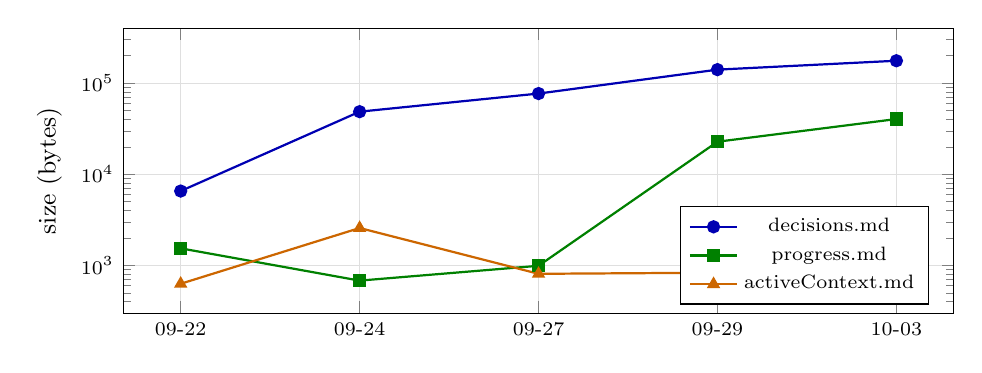
\begin{tikzpicture}
\begin{axis}[
  width=\columnwidth, height=5.2cm, ymode=log,
  symbolic x coords={09-22,09-24,09-27,09-29,10-03}, xtick=data,
  ylabel={size (bytes)}, legend pos=south east, legend style={font=\scriptsize},
  tick label style={font=\scriptsize}, label style={font=\small}, ymin=300, ymax=400000,
  enlarge x limits=0.08, grid=major, grid style={gray!25}]
\addplot[thick, mark=*, color=blue!70!black] coordinates {(09-22,6549)(09-24,48616)(09-27,76829)(09-29,140560)(10-03,175966)};
\addplot[thick, mark=square*, color=green!50!black] coordinates {(09-22,1541)(09-24,682)(09-27,992)(09-29,22761)(10-03,40358)};
\addplot[thick, mark=triangle*, color=orange!80!black] coordinates {(09-22,630)(09-24,2575)(09-27,810)(09-29,833)(10-03,887)};
\legend{decisions.md, progress.md, activeContext.md}
\end{axis}
\end{tikzpicture}
\caption{Size of the three main memory-bank files at sampled commits (log scale). The scratchpad stays flat, the decision log grows without bound, and \code{progress.md} drifted into a history.}
\label{fig:growth}
\end{figure}

\paragraph{The friction log.} Twenty-nine entries were written between 2026-09-29 and 2026-10-03, all now fixed. By area: webnav 12, codenav 8, shared MCP code 4, tooling 3, docs 2. By severity: confusing 15, wrong-result 8, blocked 3, missing-feature 2, slow 1. It is a small but complete bug tracker for the agent's own tools; one entry is the thread-bound SQLite failure of \jevmem{} itself (\S\ref{sec:eng}).

\paragraph{The \jevmem{} store.} The SpaceMaker database holds 79 notes in one scope (the largest id is 82: three notes were forgotten), of 189 characters on average (maximum 384; a decision-log entry averages about 1.4\,KB). They are linked by 657 edges (temporal 335, semantic 150, entity 143, causal 29) over 49 distinct entities. Three are pinned, three are superseded and the synthesis queue holds a resolved \emph{promote} proposal and six dismissed proposals of the (since removed) merge kind. All notes were created on 2026-10-03, while the facts they state are dated 2026-09-26 to 2026-10-02: the store was bootstrapped from the existing history, which also explains why the branch field is empty on every note.

\paragraph{A decision made because of a failure.} The decision of 2026-10-03, ``Three-way split between memory bank, \jevmem{} and \code{AGENTS.md}'', records its trigger: the store ``had picked up a copy of \code{activeContext.md}'s next steps and restatements of \code{AGENTS.md} rules''. We still find residue: note 1 is the tabs-indentation rule, explicitly marked as a hard rule in \code{AGENTS.md}, and note 10 restates the phase-gate rule. The decision was written to six places (instruction file, \code{memory/README.md}, the root README, two skills and \jevmem's README) and \emph{enforced in code} (status screen, instruction-file skip), which we regard as the more durable half.

\paragraph{Observed limits in the field.} (i) Every note has an empty branch field, so branch-aware ranking has done nothing here yet; a per-branch scope is the open item recorded in \code{activeContext.md}. (ii) The restatement filter misses some paraphrases (\S\ref{sec:eval}). (iii) The gap between the rule (``open items only'') and practice in \code{progress.md} shows that conventions without checks decay.
